%%%%%%%%%%%%%%%%%%%%%%%%%%%%%%%%%%%%%%%%%
% Short Sectioned Assignment
% LaTeX Template
% Version 1.0 (5/5/12)
%
% This template has been downloaded from:
% http://www.LaTeXTemplates.com
%
% Original author:
% Frits Wenneker (http://www.howtotex.com)
%
% License:
% CC BY-NC-SA 3.0 (http://creativecommons.org/licenses/by-nc-sa/3.0/)
%
%%%%%%%%%%%%%%%%%%%%%%%%%%%%%%%%%%%%%%%%%

%----------------------------------------------------------------------------------------
%   PACKAGES AND OTHER DOCUMENT CONFIGURATIONS
%----------------------------------------------------------------------------------------

\documentclass[paper=a4, fontsize=11pt]{scrartcl} % A4 paper and 11pt font size

\usepackage{scalefnt}
\usepackage{wrapfig}
\usepackage{graphicx}
\usepackage{subfig}



\usepackage[brazilian]{babel}
\usepackage[utf8]{inputenc}
\usepackage[T1]{fontenc}
\usepackage{amsmath,amsfonts,amsthm,mathtools} % Math packages
\usepackage{xspace}
\usepackage{indentfirst}
\usepackage{placeins}

\usepackage{url}

\usepackage{listings}
\renewcommand\lstlistingname{Algoritmo}
\lstset{ %
  numbers=left,  
  firstnumber=1,
  numberfirstline=true
  backgroundcolor=\color{white},   % choose the background color
  basicstyle=\ttfamily\scriptsize,        % size of fonts used for the code
  breaklines=true,                 % automatic line breaking only at whitespace
  captionpos=b,                    % sets the caption-position to bottom
  commentstyle=\color{mygreen},    % comment style
  escapeinside={\%*}{*)},          % if you want to add LaTeX within your code
  keywordstyle=\color{blue},       % keyword style
  stringstyle=\color{mymauve},     % string literal style
}

\usepackage{enumitem}
\setenumerate{noitemsep}

\usepackage{tikz}
\usetikzlibrary{arrows}
\usetikzlibrary{positioning}
\usetikzlibrary{calc}
\usetikzlibrary{chains}
\usetikzlibrary{shapes.multipart}

\newcommand{\snode}[2]{\node(#1)[item]{\ensuremath{#2}}}
\newcommand{\inode}[2]{\node(#1)[item, dashed]{\ensuremath{#2}}}
\newcommand{\gnode}[2]{\node(#1)[item, fill=gray]{\ensuremath{#2}}}
\newcommand{\nodelabel}[1]{\node[label]{\ensuremath{S_#1}}}

\usepackage{fancyhdr}
\pagestyle{fancyplain}
%\fancyhead{}
\fancyfoot[L]{}                      % Empty left footer
\fancyfoot[C]{}                      % Empty center footer
\fancyfoot[R]{\thepage}              % Page numbering for right footer
\renewcommand{\headrulewidth}{0pt}   % Remove header underlines
\renewcommand{\footrulewidth}{0pt}   % Remove footer underlines
\setlength{\headheight}{13.6pt}      % Customize the height of the header


\bibliographystyle{apalike}
%\bibliographystyle{alpha}

\newtheorem{theorem}{Teorema}
\newtheorem{definition}{Definição}
\newtheorem{property}{Propriedade}
\newtheorem{proposition}{Proposição}
\newtheorem{lemma}[theorem]{Lema}
\newtheorem{corollary}[theorem]{Corolário}

\numberwithin{equation}{section}
\numberwithin{figure}{section}
\numberwithin{table}{section}
\numberwithin{definition}{section}
\numberwithin{theorem}{section}
\numberwithin{property}{section}
\numberwithin{proposition}{section}


\newcommand{\horrule}[1]{\rule{\linewidth}{#1}} % horizontal rule command

\title{ 
\normalfont \small 
\textsc{DCC-IME-USP Tópicos de Análise de Algoritmos \\ Professor Fernando Mário de Oliveira Filho} \\ [25pt]
\huge Skip Lists% The assignment title
%\horrule{1pt} \\[0.5cm] % Thick bottom horizontal rule
}

\newcommand{\cP}{\ensuremath{\mathcal{P}}}
\newcommand{\cNP}{\ensuremath{\mathcal{NP}}}
\newcommand{\cO}{\ensuremath{\mathcal{O}}}
\newcommand{\Ps}{\ensuremath{\mathcal{P}_S}}

\newcommand{\SL}{\textit{Skip List}\xspace}
\newcommand{\SLs}{\textit{Skip Lists}\xspace}
\newcommand{\Sl}{\textit{Skip list}\xspace}
\newcommand{\sls}{\textit{skip lists}\xspace}
\newcommand{\skl}{\textit{skip list}\xspace}
\renewcommand{\sl}{\textit{skip list}\xspace}

\renewcommand{\bar}[1]{\overline{#1}}

\newcommand{\Exp}{\ensuremath{{\mathbb{E}}}\xspace}

\author{Gláucio Alves de Oliveira \\ Thales A. B. Paiva 
        \\ \scriptsize \{glaucioaorj, thalespaiva\}@gmail.com}
\date{\normalsize\today}

\begin{document}

\maketitle % Print the title
%\horrule{1pt} \\[0.5cm] % Thick bottom horizontal rule

\begin{abstract} \noindent

Resumimos os principais resultados sobre Skip Lists aleatorizadas (e em breve determinísticas). 
Skip Lists foram introduzidas por W. Pugh como alternativa às árvores balanceadas. 
Seu uso é justificado pelos algoritmos mais eficientes e de fácil implementação.

\end{abstract}

\tableofcontents


\section{Introdução}

Introduzidas por Pugh \cite{pugh1990skip}, \sls são uma extensão natural de listas ligadas ordenadas. 
Ambas podem ser usadas para manter um conjunto ordenado de chaves, e eventualmente seus valores associados.
Mostramos nas próximas seções que as operações de busca, inserção, e remoção em \sls são competitivas 
contra as respectivas para árvores balanceadas de busca.
Isso faz com que a escolha entre usar \sls ou árvores balanceadas numa
determinada aplicação seja baseada nas dificuldades de implementação, no uso de memória, e no tamanho das 
constantes multiplicativas dos custos de operação. 

Uma \sl consiste em um conjunto de nós, que têm chave e dados associados, e um conjunto de apontadores 
com origem em nós de chave menor, e destino em nós de chave maior.
Enquanto nas listas ligadas, um nó aponta a um só outro nó, em \sls, um nó pode apontar a vários 
outros nós de chave maior. 

A interface de operações básicas permitidas sobre uma lista ligada é a mesma que a interface
para árvores de busca:

\begin{itemize}
%  \item \textsc{Init}($p$): Cria uma \skl com parâmetro $p$ vazia e a devolve.
  \item \textsc{Insert}($S$, $k$, $d$): Insere um nó de chave $k$, e conjunto de dados
                                                 $d$, em $S$.
  \item \textsc{Remove}($S$, $k$): Remove o nó de chave $k$ de $S$.
  \item \textsc{Search}($S$, $k$): Busca o nó de chave $k$ em $S$ e o devolve.
\end{itemize}

A Figura~\ref{fig:skiplist} mostra um exemplo de \skl. 
O nó de chave $-\infty$ indica o começo da lista, e o nó de chave $+\infty$ indica o final.
Note também que cada nível de 0 a 3, representado por cada $S_0, \ldots, S_3$, forma uma lista ligada ordenada.

Os dois tipos de \sls são probabilísticas e determinísticas. Primeiro Pugh apresentou 
as probabilísticas \cite{pugh1990skip} como alternativa probabilísticas alternativas
a árvores balanceadas. Embora de implementação simples, e de ter custo médio de operações logarítmico, 
as operações em \sls probabilísticas têm alto custo no pior caso. Assim, Munro, Papadakis e 
Sedgewick propõe \sls determinísticas \cite{munro1992deterministic} que, através de algoritmos de balanceamento, mantêm o custo
logarítmico das operações, mesmo no pior caso.

Nas próximas seções, apresentamos as \sls em ordem cronológica. 

\begin{figure}
  \centering
    %extracted from https://github.com/mhyee/latex-examples/    
    \begin{tikzpicture}[
        start chain,
        every node/.style={font=\small},
        item/.style={rectangle,minimum height=7mm,minimum width=10mm,
                     rounded corners=1mm,thick,draw=black},
        label/.style={rectangle,minimum size=6mm}
      ]
      

      % The nodes of the skip list are drawn in a matrix
      % \\ delimits the rows while & delimits the columns
      \matrix[row sep=-0.2mm, column sep=5mm]{
        % Row 3: -infty ... +infty
        \nodelabel{3}; & \snode{3a}{-\infty}; & & & & & & & \snode{3h}{+\infty};\\

        % Row 2: -infty ... 6 ... 24 ... +infty
        \nodelabel{2}; & \snode{2a}{-\infty}; & & \snode{2c}{6}; & & \snode{2e}{24}; & & & \snode{2h}{+\infty};\\

        % Row 1: -infty ... 6 16 24 31 ... +infty
        \nodelabel{1}; & \snode{1a}{-\infty}; & & \snode{1c}{6}; & \snode{1d}{16}; & \snode{1e}{24}; & \snode{1f}{31}; & & \snode{1h}{+\infty};\\

        % Row 0: -infty 5 6 16 24 31 39 +infty
        \nodelabel{0}; & \snode{0a}{-\infty}; & \snode{0b}{5}; & \snode{0c}{6}; & \snode{0d}{16}; & \snode{0e}{24}; & \snode{0f}{31}; & \snode{0g}{39}; & \snode{0h}{+\infty};\\
      };

      % Start chaining the nodes together
      {
        % Horizontal chains
        % Specify a starting node (by ID), and join to other nodes (by going "through" them in an unbroken line)
        % Eg row 2: Start at 2a, join 2e, join 2h, join 2i
        [start chain] \chainin(0a); \chainin(0b) [join=by {->}]; \chainin(0c) [join=by {->}]; \chainin(0d) [join=by {->}]; \chainin(0e) [join=by {->}]; \chainin(0f) [join=by {->}]; \chainin(0g) [join=by {->}]; \chainin(0h) [join=by {->}];
        [start chain] \chainin(1a); \chainin(1c) [join=by {->}]; \chainin(1d) [join=by {->}]; \chainin(1e) [join=by {->}]; \chainin(1f) [join=by {->}]; \chainin(1h) [join=by {->}];
        [start chain] \chainin(2a); \chainin(2c) [join=by {->}]; \chainin(2e) [join=by {->}]; \chainin(2h) [join=by {->}];
        [start chain] \chainin(3a); \chainin(3h) [join=by {->}];
      }
    \end{tikzpicture}
  \caption{Exemplo de skip list.}
  \label{fig:skiplist}
\end{figure}


Estamos prontos para dar uma definição mais precisa de \sls. A definição apresentada não é 
diretamente implementável em computadores, pois usa conjuntos infinitos. Foi
parcialmente baseada na dissertação de mestrado de Mendes \cite{mendes2008estruturas}.

\begin{definition}
Uma \textbf{\emph{Skip List}} de elementos inteiros $c_1, c_2, \ldots, c_n$, 
em ordem crescente é um conjunto S tal que:

\begin{itemize}

\item $S = \{S_0, S_1, S_2, \ldots \}$ são os níveis da \sl.

\item $S_0 = \langle -\infty, c_1, c_2, \ldots, c_n, \infty \rangle.$

\item $\{-\infty, \infty\} \subseteq S_i \ $ para todo $i$.

\item Cada $S_i$, para $i \geq 1$, é um subconjunto ordenado do conjunto $S_{i-1}$, tal que:
$$
c \notin S_i \Rightarrow c_i \notin S_{i + 1}.
$$

\end{itemize}

\end{definition}


\begin{definition}

A \textbf{altura de um nó} $c$ de uma \sl $S$, denotada por $h(c)$ é o número de conjuntos de $S$ 
a que $c$ pertence.

\end{definition}

No exemplo da Figura~\ref{fig:skiplist}, $h(16) = 2$.

\begin{definition}

A \textbf{altura de uma de uma \sl} $S$, denotada por $h(S)$ é a maior altura de seus elementos finitos.
Simbolicamente
$$
h(S) = \max \{ h(c) : c \in S_0, c \notin \{ -\infty, \infty \} \}.
$$

\end{definition}

No exemplo da Figura~\ref{fig:skiplist}, $h(S) = 3$.


\pagebreak
\section{\SLs Probabilísticas}
\FloatBarrier

\subsection{Definição}

Numa \sl probabilística, o número máximo de nós a que um nó pode apontar é definido 
aleatoriamente quando este é inserido na lista, e é chamado de nível do nó.
Na definição do nível de um nó, usa-se um algoritmo que garante que, em média, a proporção 
de nós com ao menos $i + 1$ níveis em relação àqueles com ao menos $i$ níveis, seja de $p$, uma probabilidade
fixada na criação da \sl.

Na instanciação de uma \sls, é passada uma probabilidade $p$, usada na criação dos nós dessa \sl.
Assim, a adicionamos a seguinte operação à interface dessa estrutura de dados:

\begin{itemize}
  \item \textsc{Init}($p$): Cria uma \skl com parâmetro $p$ vazia e a devolve.
\end{itemize}

A definição formal de \sl probabilística é dada a seguir.

\begin{definition}
Uma \textbf{\emph{Skip List} probabilística} de elementos inteiros $c_1, c_2, \ldots, c_n$, 
em ordem crescente é um par $\left( S, p \right)$ tal que:

\begin{itemize}

\item $S = \{S_0, S_1, S_2, \ldots \}$ é uma \sl.

\item Cada $S_i$, para $i \geq 1$, é um subconjunto ordenado do conjunto $S_{i-1}$, 
construído de forma que:
  \begin{enumerate}[noitemsep]
    \item $\Pr(c \in S_i | c \in S_{i-1} ,\  c \notin \{-\infty, \infty\}) = p$.
    \item  $\Pr(c \in S_i | c \notin S_{i-1}, \ c \notin \{-\infty, \infty\}) = 0$.
  \end{enumerate}

\end{itemize}

\end{definition}


A seguir, provamos um lema simples que nos ajuda a demonstrar fatos interessantes sobre os custos das
operações em \sls probabilísticas.
\begin{lemma} \label{lemma:prob_of_node_height}
 Numa \sl $(S, p)$, a probabilidade de um nó ter altura maior ou igual a $k$ é $p^{k - 1}$.

\end{lemma}

\begin{proof}
Seja $H_N$ a variável aleatória que representa a altura de um nó. Temos, da definição de \sl:
\begin{align*}
\Pr(H_N \geq k | H_N \geq k - 1) &= p \\
\frac{\Pr(H_N \geq k \land H_N \geq k - 1)}{\Pr(H_N \geq k - 1)} &= p  \\
\frac{\Pr(H_N \geq k)}{\Pr(H_N \geq k - 1)} &= p  \\
\Pr(H_N \geq k) &= p \Pr(H_N \geq k - 1).
\end{align*}

Como temos o caso base $\Pr(H_N \geq 1) = 1 = p^0$
$$
\Pr(H_N \geq k) = p^{k - 1}.
$$
\end{proof}

\subsection{Estruturas} \label{sec:estrut}



\subsubsection{Nós}

Como uma \skl é composta por nós, primeiro vamos definir a estrutura \verb|Node|:

\begin{lstlisting}[language=C]
typedef struct node_s {
    int key;
    int height;
    struct node_s **levels;
} Node;
\end{lstlisting}

Os atributos de uma instância \verb|node| são tais que:
\begin{itemize}[noitemsep]
  \item \verb|node.key| : é a chave do nó, que é única para cada nó de uma \skl.
  \item \verb|node.height| : é o número de níveis atribuído ao nó em sua criação.
  \item \verb|node.levels[i]| : é o nó para que \verb|node| aponta em seu \verb|i|-ésimo nível.
\end{itemize}

Opcionalmente, podemos ter um atributo \verb|value|, com os valores associados a cada nó. Porém, como esse
atributo não muda em nada os algoritmos, não o consideramos.

\subsubsection{\SLs}
Agora podemos definir a estrutura \verb|SkipList|:
\begin{lstlisting}[language=C]
typedef struct skiplist_t {
    double p;
    int height;
    Node *header;
    Node *end;
} SkipList;
\end{lstlisting}

Abaixo, as descrições dos atributos de uma instância \verb|skiplist| que representa a 
\skl $( S, p )$:

\begin{itemize}[noitemsep]
  \item \verb|skiplist.p| : é a probabilidade $p$.
  \item \verb|skiplist.height| : é o nível do maior nó, e pode variar a cada inserção.
  \item \verb|skiplist.header| : é o primeiro nó da \sl com chave $-\infty$.
  \item \verb|skiplist.end| : é o último nó da \sl com chave $+\infty$.
\end{itemize}


\subsection{Algoritmos}

Nesta seção, descrevemos os algoritmos para as operações de \sls. Optamos por usar a linguagem C no lugar de 
pseudocódigo pois os algoritmos usam muitos vetores e ponteiros, então um pseudo-código teria a sintaxe muito parecida com
C, mas sem a óbvia vantagem de ser compilável. Os algoritmos implementados são exatamente os apresentados pelo
Pugh \cite{pugh1990skip}. Algumas ideias de estruturas e implementação vieram com ajuda de \cite{goodrich2014data}.

Todo o código mostrado nas próximas seções foi testado e está funcional. Uma implementação completa pode ser vista 
em: \url{github.com/thalespaiva/topalgo/blob/master/skiplist/skiplist.c}.
  
\subsubsection{Inicialização}

A inicialização de um nó é bem simples. Atribuimos os valores de sua chave, sua altura, e alocamos espaço
para os ponteiros dos seus níveis. Note que a altura não é gerada aleatoriamente nessa função.
\begin{lstlisting}[caption=Inicialização de um nó., language=C]
void node_init(Node *node, int key, int height) {
    node->key = key;
    node->height = height;

    node->levels = malloc(height*sizeof(*(node->levels)));
}
\end{lstlisting}

A inicialização da \sl cria uma lista de altura $1$ com dois nós. Um nó cabeça de chave $-\infty$ e um nó final de
chave $-\infty$. O nó cabeça tem altura como a máxima permitida mas apenas o primeiro nível é inicializado. O nó final pode 
ter altura $0$ pois é um nó sentinela e não aponta para nenhum outro.

\begin{lstlisting}[caption=Inicialização de uma skip list., language=C]
void skiplist_init(SkipList *skiplist, double p) {
    skiplist->p = p;

    skiplist->header = malloc(sizeof(*(skiplist->header)));
    skiplist->end = malloc(sizeof(*(skiplist->end)));

    node_init(skiplist->header, NEG_INF, SKIPLIST_MAX_HEIGHT);
    node_init(skiplist->end, INF, 0);

    skiplist->height = 1;
    skiplist->header->levels[0] = skiplist->end;
}
\end{lstlisting}

Na Seção~\ref{sec:ins}, descrevemos o algoritmo de inserção que usa uma função para gerar alturas pseudo-aleatórias de nós. Uma
possível implementação para esta função é dada abaixo. 
Seu funcionamento é bem simples.

\begin{lstlisting}[caption=Geração de alturas., language=C]
int skiplist_get_random_node_height(SkipList *skiplist) {
    int height;

    height = 1;
    while (rand()/(1.0 +  RAND_MAX) < skiplist->p)
        height++;

    if (height > SKIPLIST_MAX_HEIGHT)
        height = SKIPLIST_MAX_HEIGHT;
    return height;
}
\end{lstlisting}

\FloatBarrier
\subsubsection{Busca}

O algoritmo de busca por um elemento genérico de chave $k$ numa \skl faz o seguinte:
\begin{enumerate}
  \item Percorre o nível mais alto possível até encontrar um apontador para um nó de chave maior ou igual
a $k$.
  \item Quando o próximo nó tem chave maior ou igual a $k$, desce um nível na busca.
  \item Volta para o passo $1$ até que o nível de busca seja $0$.
  \item Quando o nível for $0$, estamos olhando para o nó de maior chave, dentre os nós de chave 
  menor ou igual a $k$. Então, se o próximo elemento tiver chave $k$, devolva-o. Senão devolva \verb|NULL|.
\end{enumerate}

A Figura~\ref{fig:sl_search} mostra o caminho da busca pelo elemento 31.

\begin{figure}
  \centering
    %extracted from https://github.com/mhyee/latex-examples/    
    \begin{tikzpicture}[
        start chain,
        every node/.style={font=\small},
        item/.style={rectangle,minimum height=7mm,minimum width=10mm,
                     rounded corners=1mm,thick,draw=black},
        label/.style={rectangle,minimum size=6mm}
        every arrow/.style={thick}
      ]
      \matrix[row sep=-0.2mm, column sep=5mm]{
        \nodelabel{3}; & \snode{3a}{-\infty}; & & & & & & & \snode{3h}{+\infty};\\
        \nodelabel{2}; & \snode{2a}{-\infty}; & & \snode{2c}{6}; & & \snode{2e}{24}; & & & \snode{2h}{+\infty};\\
        \nodelabel{1}; & \snode{1a}{-\infty}; & & \snode{1c}{6}; & \snode{1d}{16}; & \snode{1e}{24}; & \snode{1f}{31}; & & \snode{1h}{+\infty};\\
        \nodelabel{0}; & \snode{0a}{-\infty}; & \snode{0b}{5}; & \snode{0c}{6}; & \snode{0d}{16}; & \snode{0e}{24}; & \snode{0f}{31}; & \snode{0g}{39}; & \snode{0h}{+\infty};\\
      };

      {
        [start chain] \chainin(0a); \chainin(0b) [join=by {->}]; \chainin(0c) [join=by {->}]; \chainin(0d) [join=by {->}]; \chainin(0e) [join=by {->}]; \chainin(0f) [join=by {->}]; \chainin(0g) [join=by {->}]; \chainin(0h) [join=by {->}];
        [start chain] \chainin(1a); \chainin(1c) [join=by {->}]; \chainin(1d) [join=by {->}]; \chainin(1e) [join=by {->}]; \chainin(1f) [join=by {->}]; \chainin(1h) [join=by {->}];
        [start chain] \chainin(2a); \chainin(2c) [join=by {->}]; \chainin(2e) [join=by {->}]; \chainin(2h) [join=by {->}];
        [start chain] \chainin(3a); \chainin(3h) [join=by {->}];
      }
      {
        \path[every node/.style={font=\sffamily\small}]
        (3a.east) edge[dashed, o-, bend left] node [below] {} (2a.east)
        (2a.east) edge[dashed,  -, bend left] node [below] {} (2c.north)
        (2c.east) edge[dashed,  -, bend left] node [below] {} (2e.north)
        (2e.east) edge[dashed,  -, bend left] node [below] {} (1e.east)
        (1e.east) edge[dashed,  -, bend left] node [below] {} (0e.east)
        (0e.east) edge[dashed,  -o, bend left] node [below] {} (0f.west);
      }
    \end{tikzpicture}
  \caption{Caminho da busca pela chave $31$.}
  \label{fig:sl_search}
\end{figure}

Note que qualquer busca encontra sempre o maior nível do nó de maior chave, dentre os que têm chave menor que a
procurada. No nosso exemplo, esse nó é o de chave 24, e a busca encontrou o seu nível 2. Sugerimos que o leitor
se familiarize com o algoritmo de busca, pois ele será usado nos algoritmos de inserção e remoção.

O código em C é dado a seguir.
\begin{lstlisting}[caption=Busca., language=C]
Node *skiplist_search(SkipList *skiplist, int key) {
    int i;
    Node *tmp_node;

    tmp_node = skiplist->header;
    for (i = skiplist->height - 1; i >= 0; i--) {
        while (tmp_node->levels[i]->key < key) %* \label{line:search_cost} *)
            tmp_node = tmp_node->levels[i];
    }

    if (tmp_node->levels[0]->key == key)
        return tmp_node->levels[0];

    return NULL;
}
\end{lstlisting} \FloatBarrier

\subsubsection{Inserção} \label{sec:ins}

A inserção de um nó $k$ é ligeiramente mais complicada que a busca. Além de buscar a posição da chave $k$,
deve-se fazer com que todos os nós que vêm logo antes em cada nível apontem para o novo nó.

Para isso, enquanto a busca pelo maior nó de chave menor que $k$ é feita, o algoritmo mantém um vetor 
\verb|pointing_key_node| tal que:

\begin{center}
\verb|pointing_key_node[i]| contém o maior nó de chave menor que $k$ no nível \verb|i|.
\end{center}

Ou seja, \verb|pointing_key_node| contém os nós que, ao final da inserção, apontarão ao novo nó, em cada nível.
Note que os nós em \verb|pointing_key_node[i]| não são considerados quando 
\verb|i| maior ou igual à altura do novo nó.

Uma inserção pode aumentar a altura da \sl de $h_1$ para $h_2$. Então o algoritmo deve garantir que os níveis
entre $h_1$ e $h_2$ da cabeça da \sl apontem para os respectivos do novo nó.

Como exemplo, considere a Figura~\ref{fig:sl_insert} que trata da inserção de um nó de chave $33$. Os elementos
de \verb|pointing_key_node| são os retângulos cinza.


\begin{figure}
  \centering
    \begin{tikzpicture}[
        start chain,
        every node/.style={font=\small},
        item/.style={rectangle,minimum height=7mm,minimum width=10mm,
                     rounded corners=1mm,thick,draw=black},
        label/.style={rectangle,minimum size=6mm}
        every arrow/.style={thick}
      ]
      
      \matrix[row sep=-0.2mm, column sep=5mm]{
        \nodelabel{3}; & \gnode{3a}{-\infty}; & & & & & & & & \snode{3h}{+\infty};\\
        \nodelabel{2}; & \snode{2a}{-\infty}; & & \snode{2c}{6}; & & \gnode{2e}{24}; & & \inode{2I}{33}; & & \snode{2h}{+\infty};\\
        \nodelabel{1}; & \snode{1a}{-\infty}; & & \snode{1c}{6}; & \snode{1d}{16}; & \snode{1e}{24}; & \gnode{1f}{31}; & \inode{1I}{33};  & & \snode{1h}{+\infty};\\
        \nodelabel{0}; & \snode{0a}{-\infty}; & \snode{0b}{5}; & \snode{0c}{6}; & \snode{0d}{16}; & \snode{0e}{24}; & \gnode{0f}{31}; & \inode{0I}{33}; & \snode{0g}{39}; & \snode{0h}{+\infty};\\
      };

      {
        [start chain] \chainin(0a); \chainin(0b) [join=by {->}]; \chainin(0c) [join=by {->}]; \chainin(0d) [join=by {->}]; \chainin(0e) [join=by {->}]; \chainin(0f) [join=by {->}];  \chainin(0I) [join=by {->}]; \chainin(0g) [join=by {->}]; \chainin(0h) [join=by {->}];
        [start chain] \chainin(1a); \chainin(1c) [join=by {->}]; \chainin(1d) [join=by {->}]; \chainin(1e) [join=by {->}]; \chainin(1f) [join=by {->}];  \chainin(1I) [join=by {->}]; \chainin(1h) [join=by {->}];
        [start chain] \chainin(2a); \chainin(2c) [join=by {->}]; \chainin(2e) [join=by {->}];  \chainin(2I) [join=by {->}]; \chainin(2h) [join=by {->}];
        [start chain] \chainin(3a); \chainin(3h) [join=by {->}];
      }
      {
       \path[every node/.style={font=\sffamily\small}]
        (3a.east) edge[dashed, o-, bend left] node [below] {} (2a.east)
        (2a.east) edge[dashed,  -, bend left] node [below] {} (2c.north)
        (2c.east) edge[dashed,  -, bend left] node [below] {} (2e.north)
        (2e.east) edge[dashed,  -, bend left] node [below] {} (1e.east)
        (1e.east) edge[dashed,  -, bend left] node [below] {} (1f.north)
        (1f.east) edge[dashed,  -o, bend left] node [below] {} (0f.east);
      }
    \end{tikzpicture}
  \caption{Inserção de um nó de chave $33$.}
  \label{fig:sl_insert}
\end{figure}

Abaixo, o algoritmo em C. 

\begin{lstlisting}[caption=Inserção., language=C]
void skiplist_insert(SkipList *skiplist, int key) {
    int i;
    Node *key_node;
    Node *tmp_node;
    Node *pointing_key_node[SKIPLIST_MAX_HEIGHT];

    tmp_node = skiplist->header;                         %* \label{line:ins_beg_p1} *)
    for (i = skiplist->height - 1; i >= 0; i--) {
        while (tmp_node->levels[i]->key < key)
            tmp_node = tmp_node->levels[i];
        pointing_key_node[i] = tmp_node;
    }                                                    

    tmp_node = tmp_node->levels[0];
    if (tmp_node->key == key)
        return;                                           %* \label{line:ins_end_p1} *)

    key_node = malloc(sizeof(*key_node));
    node_init(key_node, key, skiplist_get_random_node_height(skiplist));

    if (key_node->height > skiplist->height) {            %* \label{line:ins_beg_p2} *)
        for (i = skiplist->height; i < key_node->height; i++) {
            pointing_key_node[i] = skiplist->header;
            skiplist->header->levels[i] = skiplist->end;
        }
        skiplist->height = key_node->height;
    }                                                      %* \label{line:ins_end_p2} *)

    for (i = 0; i < key_node->height; i++) {                      %* \label{line:ins_beg_p3} *)
        key_node->levels[i] = pointing_key_node[i]->levels[i];
        pointing_key_node[i]->levels[i] = key_node;
    }                                                            %* \label{line:ins_end_p3} *)
}
\end{lstlisting}

\subsubsection{Remoção}

A remoção é análoga à Inserção. Para remover um nó $c$, primeiro encontra os nós que apontam a
$c$ em cada nível. Depois, faz o nível $i$ de cada um desses nós apontar ao nó que $c$ aponta no nível $i$.
No final, libera a memória ocupada pelo nó removido.

\begin{lstlisting}[caption=Remoção., language=C]
void skiplist_remove(SkipList *skiplist, int key) {
    int i;
    Node *tmp_node;
    Node *pointing_key_node[SKIPLIST_MAX_HEIGHT];

    tmp_node = skiplist->header;
    for (i = skiplist->height - 1; i >= 0; i--) {
        while (tmp_node->levels[i]->key < key)
            tmp_node = tmp_node->levels[i];
        pointing_key_node[i] = tmp_node;
    }

    tmp_node = tmp_node->levels[0];
    if (tmp_node->key != key) 
        return;

    for (i = 0; i < skiplist->height; i++) {             %* \label{line:rem_p1} *)
        if (pointing_key_node[i]->levels[i] != tmp_node)
            break;
        pointing_key_node[i]->levels[i] = tmp_node->levels[i];
    }                                                     %* \label{line:rem_p2} *)
    free_node(tmp_node);
}

\end{lstlisting}


\subsection{Análise dos Algoritmos}

Iremos analisar cada um dos algoritmos apresentados. A estrutura da nossa análise é baseada na tese de 
mestrado de Mendes
\cite{mendes2008estruturas}, e também usamos alguns argumentos de Pugh \cite{pugh1990skip}.

\subsubsection{Inicialização}

\paragraph{Nó}
\ \\ 
Deve ser claro que a inicialização de um nó é $\cO(1)$, pois não tem laços e só faz atribuições simples.

\paragraph{\SL}
\ \\
Também deve ser claro que a inicialização de uma \SL é $\cO(1)$, pois também não tem laços e cada linha é
uma atribuição simples ou uma chamada a \verb|node_init|.

\paragraph{Geração de Alturas de Nós}
\ \\
O número esperado de operações feitas pela função \verb|skiplist_get_random_node_height| é proporcional à 
altura esperada de um nó. Assim, essa chamada tem complexidade $\cO(1/p) = \cO(1)$.

\subsubsection{Busca}

Como a função de busca é mais complicada, vamos primeiro definir o custo de uma busca.

\begin{definition}

O \textbf{custo de busca} de um elemento de uma \sl é o número de comparações feitas durante a busca por ele, sem
contar a comparação final, que testa se o nó encontrado tem a chave procurada.

\end{definition}

Assim, o custo de uma busca é o número de vezes que a comparação da linha \ref{line:search_cost} do algoritmo
de busca é executada.

Um conceito que nos ajuda a estudar o custo de buscas é o de caminho de busca. Com ele, podemos analisar o
custo de busca separadamente em seus componentes vertical e horizontal.

\begin{definition}

Um \textbf{caminho} induzido por uma busca é uma sequência $(o_1, o_2, \ldots, o_m)$ 
em que cada passo $o_i$ pertence a $\{\rightarrow, \downarrow\}$, tal que:

\begin{itemize}[noitemsep]
  \item No início da busca, a sequência é vazia.
  \item $\rightarrow$ é adicionado à sequência a cada novo nó visitado na busca.
  \item $\downarrow$ é adicionado à sequência a cada descida de nível na busca.
\end{itemize}

\end{definition}

\begin{lemma} \label{lemma:custo_busca_caminho}
O custo de busca de um elemento é igual ao tamanho do caminho de busca por esse elemento.
\end{lemma}

\begin{proof}
Cada $\rightarrow$ é adicionado pela chamada de \verb|tmp_node = tmp_node->levels[i]|, que ocorre quando a condição
\verb|tmp_node->levels[i]->key < key| é verificada. 
Cada $\downarrow$ é adicionado quando ocorre quando a condição \verb|tmp_node->levels[i]->key < key| 
não é verificada.

Logo, cada comparação adiciona um passo ao caminho de busca, e não há outro modo de adicionar um passo ao
caminho de busca.
\end{proof}

Queremos mostrar que o custo médio de busca em \sls é $\cO(\log n)$. Pelo lema~\ref{lemma:custo_busca_caminho},
podemos simplificar a demonstração dividindo a busca nas componentes vertical e horizontal.

\begin{lemma} \label{lemma:downarrow}

O número esperado de passos $\downarrow$ em qualquer caminho de busca é $\cO(\log n)$.

\end{lemma}

\begin{proof}

Note que toda busca desce até o nível 0 da \skl, então o número esperado de passos é a altura esperada, da \skl. Seja $H$ a variável aleatória que representa a altura de uma \skl $L$. E sejam 
$H_1, H_2, \ldots, H_n$ as variáveis aleatórias que representam as alturas dos elementos finitos
$c_1, c_2, \ldots, c_n$, respectivamente.

Como $H = \max \{H_i : i = 1, \ldots, n \}$, é claro que
$$
\Pr(H \geq k) \leq \sum_{i=1}^n \Pr(H_i \geq k).
$$

As $H_i$ seguem a mesma distribuição e essas variáveis são tais que, pelo Lema~\ref{lemma:prob_of_node_height},  
 $ \Pr(H_i \geq k) = p^{k - 1}$. Então
$$
\Pr(H \geq k) \leq np^{k - 1}.
$$

Como a $H$ é discreta e toma valores positivos
\begin{align*}
\Exp(H) &= \sum_{k = 0}^{\infty} \Pr(H \geq k)  \\
        &= \sum_{k = 0}^{\lceil 2 \log_{1/p} n \rceil - 1} \Pr(H \geq k) +
        \sum_{k = \lceil 2 \log_{1/p} n \rceil}^{\infty} \Pr(H \geq k).
\end{align*}

Vamos analisar cada parcela calculada. Para a primeira, temos
\begin{align*}
\sum_{k = 0}^{\lceil 2 \log_{1/p} n \rceil - 1} \Pr(H \geq k) &\leq 
  \sum_{k = 0}^{\lceil 2 \log_{1/p} n \rceil - 1} 1 \\
&\leq \lceil 2 \log_{1/p} n \rceil.
\end{align*}
E para a segunda parcela, temos
\begin{align*}
\sum_{k = \lceil 2 \log_{1/p} n \rceil}^{\infty} \Pr(H \geq k) 
   &\leq \sum_{k = \lceil 2 \log_{1/p} n \rceil}^{\infty} np^{k - 1} \\
   &= n \sum_{k = \lceil 2 \log_{1/p} n \rceil}^{\infty} p^{k - 1} \\
   &= n p^{\lceil 2 \log_{1/p} n \rceil - 1} \sum_{k = 0}^{\infty} p^k \\
   &= \frac{n}{p} p^{\lceil 2 \log_{1/p} n \rceil} \frac{1}{1 - p} \\
   &= \frac{n}{p} \left( \frac{1}{p} \right)^{- \lceil 2 \log_{1/p} n \rceil} \frac{1}{1 - p} \\
   &= \frac{n}{p} \left( \frac{1}{p} \right)^{- \lceil 2 \log_{1/p} n \rceil} \frac{1}{1 - p} \\
   &\leq \frac{n}{p} n^{-2} \frac{1}{1 - p} \\
   &= \frac{1}{np(1 - p)}.
\end{align*}

Somando os resultados
\begin{align*}
\Exp(H) &\leq \lceil 2 \log_{1/p} n \rceil + \frac{1}{np(1 - p)}.
\end{align*}

Portanto
$$
\Exp(H) = \cO(\log n).
$$
\end{proof}


\begin{lemma} \label{lemma:rightarrow}

O número esperado de passos $\rightarrow$ em qualquer caminho de busca é $\cO(\log n)$.

\end{lemma}

\begin{proof}
Considere que estamos percorrendo ao contrário um caminho de busca por um elemento $c$ qualquer 
e nos encontramos num nível qualquer de um nó que não $c$. Temos duas opções:
\begin{enumerate}[noitemsep]
  \item Se possível, subir mais um nível. 
  \item Se não, ir para a esquerda.
\end{enumerate}

Note que, se for possível subir, o caminho invertido deve subir, caso contrário, não estamos percorrendo um 
caminho válido.

A probabilidade de ser possível subir mais um nível neste nó é justamente a probabilidade de haver ao menos
$i + 1$ níveis no nó dado que há ao menos $i$ níveis, ou seja, $p$. Logo a probabilidade de termos de andar à
esquerda é $1 - p$.

Seja $R_i$ a variável aleatória que conta o número de passos $\rightarrow$ feitos no nível $i$, num 
caminho de busca. Ou seja, $R_i$ conta o número de observações \textbf{antes} de um evento com probabilidade 
$p$ ser observado. Essa interpretação mostra que $R_i \sim \text{Geom}(p)$. 

A esperança de $R_i$ é:
\begin{align*}
\Exp(R_i)
  &= \sum_{k = 1}^{\infty} k \Pr(R_i = k)= \sum_{k = 1}^{\infty} k (1 - p)^{k} p 
\end{align*}

Fazendo  $q = 1 - p$, temos
\begin{align*}
\Exp(R_i)
  &= \sum_{k = 1}^{\infty} k q^{k} (1 - q) 
    = \sum_{k = 1}^{\infty} \left( k q^{k}  - k q^{k+1} \right)  \\
  &= \sum_{k = 0}^{\infty} \left( (k+1) q^{k+1}  - k q^{k+1} \right) \\
  &= \sum_{k = 0}^{\infty} q^{k+1} 
    = \sum_{k = 1}^{\infty} q^{k}  
    = \frac{q}{1-q} \\
  &= \frac{1 - p}{p}. \\
\end{align*}

E assim, para todo nível $i$, $\Exp(R_i) = \cO(1)$.

Seja $R$ a variável aleatória que conta o número de passos $\rightarrow$ no caminho, 
e seja $H$ a variável aleatória que representa a altura da \skl. Então:
$$
R = \sum_i^H R_i.
$$

Como propriedade da esperança, temos
\begin{align*}
\Exp(R) = \Exp(\Exp(R|H)).
\end{align*}

Podemos expandir o termo $\Exp(R|H)$, obtendo
\begin{align*}
\Exp(R|H = h)
  &= \sum_{r = 1}^{\infty} r \Pr(R = r | H = h) 
   = \sum_{r = 1}^{\infty} r \Pr \left( \sum_{i=1}^{H} R_i = r | H = h \right) \\
  &= \sum_{r = 1}^{\infty} r \Pr \left( \sum_{i=1}^{h} R_i = r \right) 
   = \sum_{r = 1}^{\infty} r \Pr \left( hR_i = r \right) \\
  &= \sum_{r = 1}^{\infty} r \Pr \left( R_i = \frac{r}{h} \right)   
   = h\sum_{r = 1}^{\infty} \frac{r}{h} \Pr \left( R_i = \frac{r}{h} \right) \\
  &= h \Exp(R_i).
\end{align*}

E como $\Exp(R_i)$ não é uma variável aleatória, temos pela linearidade da esperança que
\begin{align*}
\Exp(R) = \Exp(H \Exp(R_i)) = \Exp(H)\Exp(R_i)= \cO(\log n) \cO(1).
\end{align*}

Portanto, $\Exp(R) = \cO(\log n).$

\end{proof}

\begin{theorem}
O custo médio de busca em \sls é $\cO(\log n)$. 
\end{theorem}

\begin{proof}
É corolário dos lemas \ref{lemma:downarrow} e \ref{lemma:rightarrow}. Num caminho o número de passos
é a soma do número esperado de passos $\downarrow$ com o de passos $\rightarrow$. Como ambos são
$\cO(\log n)$, a soma também é $\cO(\log n)$.
\end{proof}

\subsubsection{Inserção}

Vamos dividir o algoritmo de inserção em três partes:
\begin{enumerate}[noitemsep]
  \item Busca do maior elemento de chave menor do que a chave do nó a ser inserido, com cálculo do vetor 
    \verb|pointing_to_key_node|. Código da linha~\ref{line:ins_beg_p1} até a linha~\ref{line:ins_end_p1}.
  \item Atualização da altura da \sl, se necessário. 
      Código da linha~\ref{line:ins_beg_p2} até a linha~\ref{line:ins_end_p2}.
  \item Inserção do nó na \sl. Código da linha~\ref{line:ins_beg_p3} até a linha~\ref{line:ins_end_p3}. 
\end{enumerate}

É fácil perceber que o custo da função de inserção é composto pela soma dos custos das partes, mais a soma
de um custo constante causado pelas linhas de custo $\cO(1)$, que estão fora das partes de interesse.

\paragraph{Parte 1}
\ \\
\begin{lstlisting}[caption=Inserção Parte 1., language=C]
    tmp_node = skiplist->header;                        
    for (i = skiplist->height - 1; i >= 0; i--) {
        while (tmp_node->levels[i]->key < key)
            tmp_node = tmp_node->levels[i];
        pointing_key_node[i] = tmp_node;
    }                                                    

    tmp_node = tmp_node->levels[0];
    if (tmp_node->key == key)
        return;                                          
\end{lstlisting}

Seja $H$ novamente a variável aleatória que representa o tamanho de uma \sl.
O custo da parte 1 é o custo de uma busca mais $H$ vezes o custo de uma atualização de posição de um vetor,
que é $\cO(1)$.

Assim, seja $P_1$ o custo da parte 1. Temos que:
$$
  \Exp(P_1) = \cO(\log n) + \Exp(H) = \cO(\log n) + \cO(\log n) = \cO(\log n).
$$


\paragraph{Parte 2}
\ \\

\begin{lstlisting}[caption=Inserção Parte 2., language=C]
    if (key_node->height > skiplist->height) {            
        for (i = skiplist->height; i < key_node->height; i++) {
            pointing_key_node[i] = skiplist->header;
            skiplist->header->levels[i] = skiplist->end;
        }
        skiplist->height = key_node->height;
    }                                                      
\end{lstlisting}

Seja $P_2$ a variável aleatória que representa o custo da parte 2. $P_2$ é sempre menor ou igual ao custo no pior
caso. Sejam $H$ e $H_N$ as variáveis aleatórias que representam as alturas da \sl e do nó a ser adicionado,
respectivamente. Temos que
$$
P_2 \leq 2(H_N - H) + 1 \leq 2 H_N + 1 
$$

Então podemos afirmar, sobre o custo esperado, que
\begin{align*}
\Exp(P_2) &\leq 2\Exp(H_N) + 1 = \frac{2}{p} + 1  = \cO \left( \frac{2}{p} + 1 \right) = \cO(1).
\end{align*}


\paragraph{Parte 3}
\ \\

\begin{lstlisting}[caption=Inserção Parte 3., language=C]
    for (i = 0; i < key_node->height; i++) {                     
        key_node->levels[i] = pointing_key_node[i]->levels[i];
        pointing_key_node[i]->levels[i] = key_node;
    }                                                           
\end{lstlisting}

Sejam $P_3$ e $H_N$ as variáveis aleatórias que representam o custo da parte 3, e a altura do nó a ser
inserido. Temos que:

\begin{align*}
P_3 &= 2 H_N \\
\Exp(P_3) &= 2 \Exp(H_N) = \frac{2}{p} = \cO(1).
\end{align*}


Juntando os resultados das partes, temos que o custo esperado de uma inserção é:

\begin{align*}
\Exp(P_1 + P_2 + P_3) = \Exp(P_1) + \Exp(P_2) + \Exp(P_3) = \cO(\log n).
\end{align*}


\subsubsection{Remoção}

O algoritmo da remoção é muito parecido com o da inserção. A diferença está no trecho de código da linha~\ref{line:rem_p1}
até a linha~\ref{line:rem_p2}, copiado abaixo:
\begin{lstlisting}[caption=Parte exclusiva da Remoção, language=C]
    for (i = 0; i < skiplist->height; i++) {
        if (pointing_key_node[i]->levels[i] != tmp_node)
            break;
        pointing_key_node[i]->levels[i] = tmp_node->levels[i];
    }
    free_node(tmp_node);
\end{lstlisting}

O número de operações é proporcional à altura da \sl, que tem valor esperado $\cO(\log n)$. E a função 
que libera um nó o faz em $\cO(1)$, já que é só uma chamada a \verb|free(node->levels)|. Então, se $R$ e $I$ forem
as variáveis aleatórias que representam os custos esperados da remoção e da inserção, respectivamente, temos que,
para alguma constante $c$:
\begin{align*}
R &\leq I + c( \log n + 1) \\
\Exp(R) &\leq \Exp(I) + c( \log n + 1) = \cO(\log n) + \cO(\log n) = O(\log n).
\end{align*}


\section{\SLs Determinísticas}
\subsection{Definições}

Vimos que as operações sobre \sls têm bom custo médio. Porém, apesar de raros, os piores casos de busca,
inserção, e remoção têm custos $\cO(n)$. Como implementação alternativa de \sls que garantem
custo logarítmico até no pior caso, Munro, Papadakis, e Sedgewick, apresentaram essencialmente duas variações 
de \sls \cite{munro1992deterministic}:
\begin{itemize}
  \item 1-2 \SL;
  \item Topo-Base 1-2-3 \SL, abreviada por TB 1-2-3.
\end{itemize}

Para cada uma das duas, propuseram implementações das listas de ponteiros horizontais usando listas
ligadas e vetores. Ambas 
usam estruturas de dados parecidas, e, apesar de terem algoritmos simples para a inserção, os 
algoritmos de remoção são bem complicados, lembrando algoritmos de balanceamento de árvores balanceadas.


Neste texto, tratamos detalhadamente apenas das Topo Base 1-2-3 \SLs, por serem as mais comumente
implementadas, e ter algoritmo de balanceamento mais simples do que as 1-2 \SLs.
O motivo de as TB 1-2-3 serem mais comummente implementadas, é o fato de que
o balanceamento pode ser feito de cima para baixo, daí o nome de Topo-Base. Por ter uma implementação
mais direta, escrevemos os algoritmos usando listas ligadas para armazenar os ponteiros horizontais 
de cada nó,  pois os algoritmos ficam mais simples.

Uma TB 1-2-3 \SL é uma \sl em que, entre quaisquer nós de altura maior ou igual a $h$ consecutivos, 
há no mínimo 1, e no máximo 3, nós de altura $h - 1$. Convencionamos que os níveis dos nós 
sentinela, $-\infty$ e $+\infty$,
são de 1 a mais do que a altura da \sl. Um exemplo pode ser visto na Figura~\ref{fig:skiplist_det}.

\begin{figure}
  \centering
    %extracted from https://github.com/mhyee/latex-examples/
    \begin{tikzpicture}[
        start chain,
        every node/.style={font=\small},
        item/.style={rectangle,minimum height=7mm,minimum width=5mm,
                     rounded corners=1mm,thick,draw=black},
        label/.style={rectangle,minimum size=4mm}
      ]
      \matrix[row sep=-0.2mm, column sep=2mm]{
        \nodelabel{3}; & \snode{3neginf}{-\infty}; & & & & & & & & & & & & & & \snode{3inf}{+\infty}; \\ 
        \nodelabel{2}; & \snode{2neginf}{-\infty}; & & & & & & & \snode{2g}{64}; & & & & & & & \snode{2inf}{+\infty}; \\ 
        \nodelabel{1}; & \snode{1neginf}{-\infty}; & & & \snode{1c}{29}; & & \snode{1e}{51}; & & \snode{1g}{64}; & & & \snode{1j}{81}; & & & & \snode{1inf}{+\infty}; \\ 
        \nodelabel{0}; & \snode{0neginf}{-\infty}; & \snode{0a}{24}; & \snode{0b}{26}; & \snode{0c}{29}; & \snode{0d}{32}; & \snode{0e}{51}; & \snode{0f}{62}; & \snode{0g}{64}; & \snode{0h}{75}; & \snode{0i}{79}; & \snode{0j}{81}; & \snode{0k}{90}; & \snode{0l}{91}; & \snode{0m}{94}; & \snode{0inf}{+\infty}; \\ 
      };
      {
        [start chain] \chainin(0neginf);\chainin(0a) [join=by {->}];\chainin(0b) [join=by {->}];\chainin(0c) [join=by {->}];\chainin(0d) [join=by {->}];\chainin(0e) [join=by {->}];\chainin(0f) [join=by {->}];\chainin(0g) [join=by {->}];\chainin(0h) [join=by {->}];\chainin(0i) [join=by {->}];\chainin(0j) [join=by {->}];\chainin(0k) [join=by {->}];\chainin(0l) [join=by {->}];\chainin(0m) [join=by {->}];\chainin(0inf) [join=by {->}]; 
        [start chain] \chainin(1neginf);\chainin(1c) [join=by {->}];\chainin(1e) [join=by {->}];\chainin(1g) [join=by {->}];\chainin(1j) [join=by {->}];\chainin(1inf) [join=by {->}]; 
        [start chain] \chainin(2neginf);\chainin(2g) [join=by {->}];\chainin(2inf) [join=by {->}]; 
        [start chain] \chainin(3neginf);\chainin(3inf) [join=by {->}]; 
      }

    \end{tikzpicture}
  \caption{Exemplo de TB 1-2-3 \SL}
  \label{fig:skiplist_det}
\end{figure}


A seguir, damos uma definição formal das TB 1-2-3 \sls.

\begin{definition}
Uma \textbf{TB 1-2-3 \emph{Skip List} determinística} de elementos inteiros $c_1, c_2, \ldots, c_n$, 
em ordem crescente é um conjunto S tal que:

\begin{itemize}

\item $S = \{S_0, S_1, S_2, \ldots \}$ é uma \sl.

\item $h(-\infty) = h(+\infty) = h(S) + 1$, por definição.

\item Para todo $S_i$, com $i \geq 1$, se $c$ e $d$ são elementos consecutivos de $S_i$, então vale que:
$$
1 \leq \ \bigm| \{ x \in S_{i -1} : c < x < d \}  \bigm| \ \leq 3.
$$

\end{itemize}

\end{definition}

Como consequência da definição, temos o seguinte lema sobre a altura de uma 1-2 \sl.

\begin{lemma}
A altura de uma TD 1-2-3 \sl é $\cO(log n)$.
\end{lemma}

\begin{proof}
É fácil ver que altura máxima é atingida quando, para cada dois elementos 
consecutivos $c$ e $d$, do nível $S_i$ ($i \geq 1$), existir apenas 1 elemento $x$ de $S_{i-1}$ 
tal que $c < x < d$. Assim, para $ i \geq 1 $, temos que:
$$
|S_i| \leq \frac{|S_{i-1}|}{2} \ \ \overset{|S_0| = n}\implies \ \ |S_i| \leq \frac{n}{2^i}.
$$

Se $h$ for a altura da \sl, então $1 \leq |S_{k-1}| \leq 2$. Assim, temos que:
$$
1 \leq \frac{n}{2^h} \Rightarrow 2^h \leq n \Rightarrow h \leq \log_2(n) \Rightarrow h = \cO(\log n). 
$$
\end{proof}


\subsection{Estruturas}

Os dois tipos de \sls determinísticas usam as mesmas estruturas, definidas nas curtas seções a seguir.
Note o contraste com as \sls probabilísticas. Enquanto nelas temos a estrutura nó que representa
cada item de uma \sl, nas determinísticas temos a estrutura célula, que representa um determinado 
nível de um dado nó.

\subsubsection{Células}

\begin{lstlisting}[caption=Estrutura das Células, language=C]
typedef struct cell_t {
    int key;
    struct cell_t *down;
    struct cell_t *right;
} Cell;
\end{lstlisting}

Apesar de parecer uma estrutura familiar, comparando com as \sls probabilísticas, há uma diferença
semântica fundamental. O ponteiro \verb|down| da célula \verb|cell| do $i$-ésimo nível de um nó,
aponta para a primeira célula no nível $i - 1$ que é pulada por um ponteiro até \verb|cell|.

A Figura~\ref{fig:cell_structure} mostra a representação de uma \sl usando esses ponteiros.

\subsubsection{SkipList}
\begin{lstlisting}[caption=Estrutura das Skip Lists determinísticas, language=C]
typedef struct skiplist_t {
    Cell *header;
    Cell *end;
    Cell *bottom;
} SkipList;
\end{lstlisting}


\begin{figure}
  \centering
    %extracted from https://github.com/mhyee/latex-examples/
    \begin{tikzpicture}[
        start chain,
        every node/.style={font=\small},
        item/.style={rectangle,minimum height=7mm,minimum width=15mm,
                     rounded corners=1mm,thick,draw=black},
        label/.style={rectangle,minimum size=6mm}
      ]
      \matrix[row sep=5mm, column sep=5mm]{
        \snode{header}{header}; & & & & & \snode{2inf}{+\infty}; \\ 
        \snode{1b}{21}; & & & \snode{1mk}{MaxKey}; & & \snode{1inf}{+\infty}; \\ 
        \snode{0a}{20}; & \snode{0b}{21}; & \snode{0c}{26}; & \snode{0d}{27}; & \snode{0mk}{MaxKey}; & \snode{0inf}{+\infty}; \\ 
      };
      {
        [start chain] \chainin(0a); \chainin(0b) [join=by {->}];\chainin(0c) [join=by {->}]; \chainin(0d) [join=by {->}]; \chainin(0mk) [join=by {->}];  \chainin(0inf) [join=by {->}]; 
        [start chain] \chainin(1b); \chainin(1mk) [join=by {->}]; \chainin(1inf) [join=by {->}]; 
        [start chain] \chainin(header); \chainin(2inf) [join=by {->}]; 
        [start chain] \chainin(header); \chainin(1b) [join=by {->}]; \chainin(0a) [join=by {->}]; 
        [start chain] \chainin(1mk)  ; \chainin(0d) [join=by {->}]; 
      }
      
    \end{tikzpicture}
  \caption{Exemplo do uso da estrutura \texttt{cell}}
  \label{fig:cell_structure}
\end{figure}




\subsection{Algoritmos}

Os algoritmos mostrados nesta seção são baseados no trabalho de Munro et al.
sobre \sls determinísticas \cite{munro1992deterministic}, e também na tese de doutorado de Papadakis
\cite{papadakis1993skip}. Neste artigo, os autores descrevem 
em alto nível os algoritmos de inserção e remoção.
Pode-se ver implementações completas em 


\subsubsection{Inicialização}

A inicialização de células é bem simples. Passa-se um ponteiro de célula, uma chave, e ponteiros para
as células de baixo e à direita.

\begin{lstlisting}[caption=Inicialização de células de Skip Lists determinísticas, language=C]

void cell_init(Cell *cell, int key, Cell *bottom, Cell *right) {
    cell->key = key;
    cell->bottom = bottom;
    cell->right = right;
}

\end{lstlisting}

A inicialização de \sls é simples, mas deve-se atentar para os nós sentinelas, e os valores de 
seus atributos.

\begin{lstlisting}[caption=Inicialização de Skip Lists determinísticas, language=C]
#define INF INT_MAX

void skiplist_init(SkipList *skiplist) {
    skiplist->header = malloc(sizeof(*(skiplist->header)));
    skiplist->end = malloc(sizeof(*(skiplist->end)));
    skiplist->bottom = malloc(sizeof(*(skiplist->bottom)));

    cell_init(skiplist->bottom, INF, skiplist->bottom, skiplist->bottom);
    cell_init(skiplist->end, INF, NULL, skiplist->end);
    cell_init(skiplist->header, INF - 1, skiplist->bottom, skiplist->end);
}
\end{lstlisting}

\subsubsection{Busca}

O algoritmo de busca em \sls determinísticas é essencialmente o mesmo daquele para as probabilísticas, 
percorrendo a lista através dos ponteiros \verb|right| e \verb|bottom|.

\begin{lstlisting}[caption=Algortimo de busca para Skip Lists determinísticas, language=C]
Cell *skiplist_search(SkipList *skiplist, int key) {
    Cell *cell;

    cell = skiplist->header;

    skiplist->bottom->key = key;
    while (cell->key != key) {
        if (key < cell->key)
            cell = cell->down;
        else
            cell = cell->right;
    }
    if (cell == skiplist->bottom)
        return NULL;
    return cell;
}
\end{lstlisting}

\subsubsection{Inserção}

A inserção em \sls determinísticas é feita de modo bem elegante. Uma inserção 
começa-se na cabeça da \sl, em seu último nível. Primeiro, faz-se uma busca, naquele nível, pela chave do elemento
a ser inserido. Com isso, descobre-se qual o intervalo que conterá o novo item. Se, em seu nível abaixo,
esse intervalo contiver 3 elementos seguidos de mesmo nível, o do meio é aumentado em 1 nível.
Esse procedimento é feito a cada nível, até atingir a base da \sl. Por fim, pode-se garantidamente
inserir o elemento com altura 1.

A Figura~\ref{fig:det_skiplist_ins} exemplifica a inserção do elemento 31. Os passos são os seguintes:
\begin{itemize}
  \item Na iteração do nível 3, vê-se que não há três nós de mesma altura no nível 2. Assim, pode-se descer
  sem problemas.
  \item Na iteração do nível 2, vê-se que o intervalo em que estará o 31 é o de $-\infty$ a 64. Como este
  intervalo têm três elementos de mesma altura, no nível 1, aumenta-se o nível de 29.
  \item Na iteração do nível 1, vê-se que o intervalo em que estará o 31 é o de 29 a 37. Como não
  há três elementos de mesma altura no nível 0, pode-se descer ao nível 0.
  \item Na iteração do nível 0, coloca-se o 31 após o 29, com altura 1.
\end{itemize}

O algoritmo de inserção é dado a seguir. Pode-se ver como os nós sentinela, ao invés de ponteiros
nulos, ajudam a eliminar condicionais antes de fazer buscas de ponteiros, deixando o código mais limpo.

\begin{figure}
  \centering
    %extracted from https://github.com/mhyee/latex-examples/
    \begin{tikzpicture}[
        start chain,
        every node/.style={font=\small},
        item/.style={rectangle,minimum height=7mm,minimum width=5mm,
                     rounded corners=1mm,thick,draw=black},
        label/.style={rectangle,minimum size=5mm}
      ]
      \matrix[row sep=-0.2mm, column sep=2mm]{
        \nodelabel{3}; & \snode{3neginf}{-\infty}; & & & & & & & & & & & & & & & \snode{3inf}{+\infty}; \\ 
        \nodelabel{2}; & \snode{2neginf}{-\infty}; & & & & & & & & & & \snode{2j}{64}; & & & & & \snode{2inf}{+\infty}; \\ 
        \nodelabel{1}; & \snode{1neginf}{-\infty}; & & \snode{1b}{21}; & & \snode{1d}{29}; & & & & \snode{1h}{51}; & & \snode{1j}{64}; & & & \snode{1m}{81}; & & \snode{1inf}{+\infty}; \\ 
        \nodelabel{0}; & \snode{0neginf}{-\infty}; & \snode{0a}{20}; & \snode{0b}{21}; & \snode{0c}{26}; & \snode{0d}{29}; & \snode{0e}{32}; & \snode{0f}{37}; & \snode{0g}{48}; & \snode{0h}{51}; & \snode{0i}{62}; & \snode{0j}{64}; & \snode{0k}{75}; & \snode{0l}{79}; & \snode{0m}{81}; & \snode{0n}{90}; & \snode{0inf}{+\infty}; \\ 
      };
      {
        [start chain] \chainin(0neginf);\chainin(0a) [join=by {->}];\chainin(0b) [join=by {->}];\chainin(0c) [join=by {->}];\chainin(0d) [join=by {->}];\chainin(0e) [join=by {->}];\chainin(0f) [join=by {->}];\chainin(0g) [join=by {->}];\chainin(0h) [join=by {->}];\chainin(0i) [join=by {->}];\chainin(0j) [join=by {->}];\chainin(0k) [join=by {->}];\chainin(0l) [join=by {->}];\chainin(0m) [join=by {->}];\chainin(0n) [join=by {->}];\chainin(0inf) [join=by {->}]; 
        [start chain] \chainin(1neginf);\chainin(1b) [join=by {->}];\chainin(1d) [join=by {->}];\chainin(1h) [join=by {->}];\chainin(1j) [join=by {->}];\chainin(1m) [join=by {->}];\chainin(1inf) [join=by {->}]; 
        [start chain] \chainin(2neginf);\chainin(2j) [join=by {->}];\chainin(2inf) [join=by {->}]; 
        [start chain] \chainin(3neginf);\chainin(3inf) [join=by {->}]; 
      }

    \end{tikzpicture}


    \begin{tikzpicture}[
        start chain,
        every node/.style={font=\small},
        item/.style={rectangle,minimum height=7mm,minimum width=5mm,
                     rounded corners=1mm,thick,draw=black},
        label/.style={rectangle,minimum size=5mm}
      ]
      \matrix[row sep=-0.2mm, column sep=2mm]{
        \nodelabel{3}; & \snode{3neginf}{-\infty}; & & & & & & & & & & & & & & & & \snode{3inf}{+\infty}; \\ 
        \nodelabel{2}; & \snode{2neginf}{-\infty}; & & & & \snode{2d}{29}; & & & & & & & \snode{2k}{64}; & & & & & \snode{2inf}{+\infty}; \\ 
        \nodelabel{1}; & \snode{1neginf}{-\infty}; & & \snode{1b}{21}; & & \snode{1d}{29}; & & & \snode{1g}{37}; & & \snode{1i}{51}; & & \snode{1k}{64}; & & & \snode{1n}{81}; & & \snode{1inf}{+\infty}; \\ 
        \nodelabel{0}; & \snode{0neginf}{-\infty}; & \snode{0a}{20}; & \snode{0b}{21}; & \snode{0c}{26}; & \snode{0d}{29}; & \snode{0e}{31}; & \snode{0f}{32}; & \snode{0g}{37}; & \snode{0h}{48}; & \snode{0i}{51}; & \snode{0j}{62}; & \snode{0k}{64}; & \snode{0l}{75}; & \snode{0m}{79}; & \snode{0n}{81}; & \snode{0o}{90}; & \snode{0inf}{+\infty}; \\ 
      };
      {
        [start chain] \chainin(0neginf);\chainin(0a) [join=by {->}];\chainin(0b) [join=by {->}];\chainin(0c) [join=by {->}];\chainin(0d) [join=by {->}];\chainin(0e) [join=by {->}];\chainin(0f) [join=by {->}];\chainin(0g) [join=by {->}];\chainin(0h) [join=by {->}];\chainin(0i) [join=by {->}];\chainin(0j) [join=by {->}];\chainin(0k) [join=by {->}];\chainin(0l) [join=by {->}];\chainin(0m) [join=by {->}];\chainin(0n) [join=by {->}];\chainin(0o) [join=by {->}];\chainin(0inf) [join=by {->}]; 
        [start chain] \chainin(1neginf);\chainin(1b) [join=by {->}];\chainin(1d) [join=by {->}];\chainin(1g) [join=by {->}];\chainin(1i) [join=by {->}];\chainin(1k) [join=by {->}];\chainin(1n) [join=by {->}];\chainin(1inf) [join=by {->}]; 
        [start chain] \chainin(2neginf);\chainin(2d) [join=by {->}];\chainin(2k) [join=by {->}];\chainin(2inf) [join=by {->}]; 
        [start chain] \chainin(3neginf);\chainin(3inf) [join=by {->}]; 
      }


    \end{tikzpicture}


  \caption{Inserção do elemento 31 num TB 1-2-3 skip list.}
  \label{fig:det_skiplist_ins}
\end{figure}


\begin{lstlisting}[caption=Algoritmo de inserção em TB 1-2-3 skip list, language=C]
void skiplist_insert(SkipList *skiplist, int key) {
    int gap_last_key;
    Cell *cell, *new;

    skiplist->bottom->key = key;

    cell = skiplist->header;
    while (cell != skiplist->bottom) {

        while (key > cell->key)
            cell = cell->right;

        if ((cell->down == skiplist->bottom) && (cell->key == key))
            return;

        gap_last_key = cell->down->right->right->right->key;
        if (cell->down == skiplist->bottom || cell->key == gap_last_key) {
            new = malloc(sizeof(*new));
            cell_init(new, cell->key, cell->down->right->right, cell->right);
            cell->right = new;
            cell->key = cell->down->right->key;
        }

        cell = cell->down;
    }

    if (skiplist->header->right != skiplist->end)
        skiplist_grow(skiplist);
}

void skiplist_grow(SkipList *skiplist) {
    Cell *new_cell;

   new_cell = malloc(sizeof(*new_cell));
   cell_init(new_cell, INF - 1, skiplist->header, skiplist->end);
   skiplist->header = new_cell;
}
\end{lstlisting}


\subsubsection{Remoção}

A remoção em \sls determinísticas é mais complicada, como em árvores balanceadas. 
A ideia é similar à inserção: a cada nível, observar o nível abaixo fazendo, se necessário, algum 
balanceamento antes de descer um nível.

A remoção de um elemento começa na cabeça da list, no último nível \textbf{da skip list}. Faz-se uma busca nesse nível 
pelo intervalo em que está o elemento a ser removido. Verifica quantos elementos seguidos de mesma altura
há no nível abaixo. Se há 2 ou 3, é seguro descer, pois a remoção será segura. Se há 1, faz-se o 
balanceamento através da união com um intervalo vizinho, ou troca de altura com um elemento de
intervalo vizinho.


Considere a remoção representada na Figura~\ref{fig:det_skiplist_rem}.

\begin{itemize}
  \item Na iteração do nível 2, vê-se que 71 está entre $-\infty$ e  75. Também observa-se que, no nível
  1, há dois elementos de mesma altura seguidos, nesse intervalo. Então a descida é segura.
  \item Na iteração do nível 1, vê-se que 71 está entre 47 e 75. Nesse intervalo, há somente 1 elemento
  no nível 0. Assim, é preciso balancear para que a remoção seja segura. Como esse intervalo tem um 
  intervalo vizinho com dois elementos, toma-se o elemento mais à direita, 25, para trocar de nível com
  o 47. Assim, o novo intervalo, de 25 a 75 é seguro, e pode-se descer.
  \item Na iteração do nível 0, o elemento 71 pode ser removido com segurança.

\end{itemize}

\begin{figure}
  \centering
    %extracted from https://github.com/mhyee/latex-examples/
    \begin{tikzpicture}[
        start chain,
        every node/.style={font=\small},
        item/.style={rectangle,minimum height=7mm,minimum width=5mm,
                     rounded corners=1mm,thick,draw=black},
        label/.style={rectangle,minimum size=4mm}
      ]
      \matrix[row sep=-0.2mm, column sep=2mm]{
        \nodelabel{3}; & \snode{3neginf}{-\infty}; & & & & & & & & & & & & \snode{3inf}{+\infty}; \\ 
        \nodelabel{2}; & \snode{2neginf}{-\infty}; & & & & & & & & \snode{2h}{75}; & & & & \snode{2inf}{+\infty}; \\ 
        \nodelabel{1}; & \snode{1neginf}{-\infty}; & & & \snode{1c}{18}; & & & \snode{1f}{47}; & & \snode{1h}{75}; & & \snode{1j}{78}; & & \snode{1inf}{+\infty}; \\ 
        \nodelabel{0}; & \snode{0neginf}{-\infty}; & \snode{0a}{ 7}; & \snode{0b}{ 8}; & \snode{0c}{18}; & \snode{0d}{23}; & \snode{0e}{25}; & \snode{0f}{47}; & \snode{0g}{71}; & \snode{0h}{75}; & \snode{0i}{77}; & \snode{0j}{78}; & \snode{0k}{95}; & \snode{0inf}{+\infty}; \\ 
      };
      {
        [start chain] \chainin(0neginf);\chainin(0a) [join=by {->}];\chainin(0b) [join=by {->}];\chainin(0c) [join=by {->}];\chainin(0d) [join=by {->}];\chainin(0e) [join=by {->}];\chainin(0f) [join=by {->}];\chainin(0g) [join=by {->}];\chainin(0h) [join=by {->}];\chainin(0i) [join=by {->}];\chainin(0j) [join=by {->}];\chainin(0k) [join=by {->}];\chainin(0inf) [join=by {->}]; 
        [start chain] \chainin(1neginf);\chainin(1c) [join=by {->}];\chainin(1f) [join=by {->}];\chainin(1h) [join=by {->}];\chainin(1j) [join=by {->}];\chainin(1inf) [join=by {->}]; 
        [start chain] \chainin(2neginf);\chainin(2h) [join=by {->}];\chainin(2inf) [join=by {->}]; 
        [start chain] \chainin(3neginf);\chainin(3inf) [join=by {->}]; 
      }

    \end{tikzpicture}
    
        \begin{tikzpicture}[
        start chain,
        every node/.style={font=\small},
        item/.style={rectangle,minimum height=7mm,minimum width=5mm,
                     rounded corners=1mm,thick,draw=black},
        label/.style={rectangle,minimum size=4mm}
      ]
      \matrix[row sep=-0.2mm, column sep=2mm]{
        \nodelabel{3}; & \snode{3neginf}{-\infty}; & & & & & & & & & & & \snode{3inf}{+\infty}; \\ 
        \nodelabel{2}; & \snode{2neginf}{-\infty}; & & & & & & & \snode{2g}{75}; & & & & \snode{2inf}{+\infty}; \\ 
        \nodelabel{1}; & \snode{1neginf}{-\infty}; & & & \snode{1c}{18}; & & \snode{1e}{25}; & & \snode{1g}{75}; & & \snode{1i}{78}; & & \snode{1inf}{+\infty}; \\ 
        \nodelabel{0}; & \snode{0neginf}{-\infty}; & \snode{0a}{ 7}; & \snode{0b}{ 8}; & \snode{0c}{18}; & \snode{0d}{23}; & \snode{0e}{25}; & \snode{0f}{47}; & \snode{0g}{75}; & \snode{0h}{77}; & \snode{0i}{78}; & \snode{0j}{95}; & \snode{0inf}{+\infty}; \\ 
      };
      {
        [start chain] \chainin(0neginf);\chainin(0a) [join=by {->}];\chainin(0b) [join=by {->}];\chainin(0c) [join=by {->}];\chainin(0d) [join=by {->}];\chainin(0e) [join=by {->}];\chainin(0f) [join=by {->}];\chainin(0g) [join=by {->}];\chainin(0h) [join=by {->}];\chainin(0i) [join=by {->}];\chainin(0j) [join=by {->}];\chainin(0inf) [join=by {->}]; 
        [start chain] \chainin(1neginf);\chainin(1c) [join=by {->}];\chainin(1e) [join=by {->}];\chainin(1g) [join=by {->}];\chainin(1i) [join=by {->}];\chainin(1inf) [join=by {->}]; 
        [start chain] \chainin(2neginf);\chainin(2g) [join=by {->}];\chainin(2inf) [join=by {->}]; 
        [start chain] \chainin(3neginf);\chainin(3inf) [join=by {->}]; 
      }

    \end{tikzpicture}

  \caption{Remoção do elemento 71}
  \label{fig:det_skiplist_rem}
\end{figure}




A seguir, é dado o algoritmo para a remoção. Ele é consideravelmente mais extenso que o de inserção, 
porém, não é muito mais complicado.


\begin{lstlisting}[caption=Algoritmo de remoção em TB 1-2-3 skip list, language=C]
void skiplist_remove(SkipList *skiplist, int key) {
    Cell *current, *previous, *next, *node;
    int previous_key, last_above;

    current = skiplist->header->down;
    skiplist->bottom->key = key;
    last_above = skiplist->header->key;

    while (current != skiplist->bottom) {
        while (key > current->key) {
            previous = current;
            current = current->right;
        }
        next = current->down;

        if (current->key == next->right->key) {
            if (current->key != last_above) {
                node = current->right;
                if ((node->key==node->down->right->key) || (next==skiplist->bottom)) {
                    current->right = node->right;
                    current->key = node->key;
                    free(node);
                }
                else {
                    current->key = node->down->key;
                    node->down = node->down->right;
                }
            }
            else {
                if (previous->key <= previous->down->right->key) {
                    if (next == skiplist->bottom)
                        previous_key = previous->key;
                    previous->right = current->right;
                    previous->key = current->key;
                    free(current);
                    current = previous;
                }
                else {
                    if (previous->key == previous->down->right->right->key)
                        node = previous->down->right;
                    else
                        node = previous->down->right->right;
                    previous->key = node->key;
                    current->down = node->right;
                }
            }
        }
        last_above = current->key;
        current = next;
    }
    current = skiplist->header->down;
    while (current != skiplist->bottom) {
        while (key > current->key)
            current = current->right;
        if (key == current->key)
            current->key = previous_key;
        current = current->down;
    }

    if (skiplist->header->down->right == skiplist->end) {
        current = skiplist->header;
        skiplist->header = current->down;
        free(current);
    }
}
\end{lstlisting}


\subsection{Análise dos algoritmos}

Apesar de algoritmos mais complicados, a análise dos algoritmos mais simples para \sl determinísticas
do que para as probabilísticas. Isso pois os laços principais dos algoritmos são feitos percorrendo
a altura, que é $\cO(\log n)$, e numa busca, não se dá mais do que três passos à direita.

\subsubsection{Inicialização}

Deve ser claro que a inicialização é $\cO(1)$.

\subsubsection{Busca}

Sabemos que a altura de uma TB 1-2-3 \sl é $\cO(\log n)$. Então, no pior caso, o laço principal faz
$3 O(\log n)$ operações, pois, no máximo, são dados três passos à direita.

\subsubsection{Inserção}

O custo da inserção é dominado pelo custo da busca. Isso pois, dentro do laço principal, é fácil
ver que cada condicional tem custo $\cO(1)$, e, pelo mesmo argumento usado na análise da busca, 
o while interno faz 3 comparações no pior caso. Somando isso com o custo $\cO(1)$ da função 
\verb|skiplist_grow|, temos que o custo total da inserção é $\cO(\log n)$.

\subsubsection{Remoção}

Como na inserção, podemos desconsiderar os custos dos condicionais no laço principal da remoção pois 
não há laço ou chamada de procedimento, que não o \verb|free|, que tem custo $\cO(1)$. Assim, o
laço principal da remoção é dominado pelo custo de busca.

É claro que o \verb|while| da linha 52 tem custo igual ao de uma busca, a menos de uma constante
multiplicativa. E o condicional da linha 60 é $\cO(1)$.

Assim, o custo de remoção é $\cO(\log n) + \cO(\log n) + \cO(1) = \cO(\log n)$.



\section{An\'{a}lise do tempo de diferentes algoritmos.}

Na tabela 4.1, verifica-se o desempenho da estrutura \textit{skip list} em rela\c{c}\~{a}o a outras estruturas de dados. Segundo W.Pugh, tais algoritmos foram implementados em linguagem C. Maiores detalhes sobre a autoria dos respectivos algoritmos e infoma\c{c}\~{a}o adicional  da CPU podem ser vistos no referido trabalho de W. Pugh.  


\begin{table}[htpb]
  \centering
  
 \scalefont{0.7}
   
  \begin{tabular}{|c|c|c|c|c|c|c|c|c|c|c|c|c|c|}
  
  \hline
          Implementa\c{c}\~{a}o & Tempo de busca & Tempo de  inser\c{c}\~{a}o & Tempo de remo\c{c}\~{a}o\\
          \hline
          \textit{Skip Lists} & $0.051 mseg$ & $0.065 mseg$ & $0.059 mseg$\\
          \hline
          \'{A}rvores AVL  n\~{a}o - recursivas & $0.046 mseg$ & $0.10 mseg$ &$0.085 mseg$\\ 
          \hline
           \'{A}rvores 2 - 3 recursivas & $0.054 mseg$ & $0.21 mseg$ & $0.21 mseg$\\
           \hline
          \'{A}rvores auto-ajust\'{a}veis \textit{Top down splaying} & $0.15 mseg$ & $0.16 mseg$ & $0.18 mseg$\\
           \hline
           \'{A}rvores auto-ajust\'{a}veis \textit{Bottom-up splaying} & $0.49 mseg$ & $0.51 mseg$ & $0.53 mseg$\\
           \hline 
  \end{tabular}

 \caption{Diferentes algoritmos e respectivos tempos em \textit{milisegundos}. Retirado de [Pugh, 1990.]}
 
\end{table}


\pagebreak
\section{ \textit{Skip list} em um ambiente concorrente.}

\subsection{Contextualiza\c{c}\~{a}o}

                  Em 1990, William Pugh publicou o artigo ``Concorrent maintenance of \textit{skip lists}''. Nesse trabalho, afirmou-se que os algoritmos de \textit{skip list} aplicados no ambiente programa\c{c}\~{a}o concorrente fornecem um m\'{e}todo pr\'{a}tico de acesso e atualiza\c{c}\~{a}o em uma estrutura de pesquisa com mem\'{o}ria compartilhada. Ainda segundo o referido artigo, essa afirma\c{c}\~{a}o baseou-se no fato de que as \textit{skip lists} serem aproximadamente tao r\'{a}pidas ou mais do que as \'{a}rvores balanceadas em uma ambiente n\~{a}o concorrente e, al\'{e}m disso, problemas espec\'{i}ficos desse ambiente, tais como a ``conten\c{c}\~{a}o'', n\~{a}o impactaria significativamente no desempenho das \textit{skip lists} concorrentes. Por fim, nesse trabalho, W. Pugh acreditou que o projeto de algoritmos de \'{a}rvores balanceadas em ambientes concorrentes permitiria uma alta efici\^{e}ncia em opera\c{c}\~{o}es, contudo com uma complexidade que faria sua implementa\c{c}\~{a}o ``proibitiva''.  Desta forma, desde o inicio da d\'{e}cada de 90, W.Pugh j\'{a} vislumbrava a aplica\c{c}\~{a}o da estrutura \textit{skip list }em um ambiente de programa\c{c}\~{a}o concorrente tamb\'{e}m como uma alternativa a outras estruturas de dados. Conv\'{e}m ressaltar que, no referido artigo de William Pugh, pode ser verificado apenas um pseudo-c\'{o}digo de uma opera\c{c}\~{a}o de busca de uma \textit{skip list}  em um ambiente concorrente.
                  
  
Em 2015, na Austr\'{a}lia, mais precisamente na Universidade de Sidney, Vicente Gramoli publicou um trabalho entitulado ``More than you ever wanted to know about synchronization". O referido artigo faz um estudo comparativo entre cinco t\'{e}cnicas de sincroniza\c{c}\~{a}o aplicadas em 31 algoritmos referentes a 4 estruturas de dados consagradas. As implementa\c{c}\~{o}es foram feitas nas linguagens C/C++ e Java. Resumindo em poucas palavras, o artigo afirma que foi implementado um \textit{software} chamado \textit{synchrobench} com o prop\'{o}sito de auxiliar pesquisadores a avaliar novas estruturas de dados com t\'{e}cnicas de sincroniza\c{c}\~{a}o (lock, transaction e etc). Conv\'{e}m ressaltar que o foco desta resenha, no que tange a este t\'{o}pico,  visa a analisar de uma forma superficial o desempenho da estrutura \textit{skip list} no ambiente de programa\c{c}\~{a}o concorrente em compara\c{c}\~{a}o a outras estruturas de dados e, \textit{a priori}, n\~{a}o h\'{a} nenhuma inten\c{c}\~{a}o ou preocupa\c{c}\~{a}o dos autores desta resenha em explicar t\'{e}cnicas de  sincroniza\c{c}\~{a}o em ambiente concorrente. Adicionalmente, observa-se na tabela 5.1 apenas os algoritmos referentes as estruturas \textit{skip list} e \'{a}rvore bin\'{a}ria. Tem-se um total de 14 algoritmos sendo os 8 primeiros atinentes \`{a} estrutura de \'{a}rvores bin\'{a}rias e os 6 \'{u}ltimos \`{a} estrutura de \textit{skip list.} Para uma visualiza\c{c}\~{a}o completa das outras estruturas de dados e maiores detalhes, recomenda-se a verifica\c{c}\~{a}o do artigo de V. Gramoli.   

\begin{table}[htpb]
  \centering
  
  \scalefont{0.72}
   
  \begin{tabular}{|c|c|c|c|c|c|c|c|c|c|c|c|c|c|}
  
  \hline
          $\#$&Algorithm & Synchronization & Data structures &Language\\
          \hline
         1&Practical binary tree & lock &  binary tree&Java \\
          \hline
          2&Contention-friendly tree & lock & binary tree &Java\\ 
          \hline
           3&Logical ordering tree & lock &binary tree &Java\\
          \hline
           4&Lock-free tree& read-modify-write &binary tree&Java\\
           \hline
           5&Fast lock-free tree& read-modify-write &binary tree &C/C++\\
           \hline 
           6&Speculation-friendly tree & transaction &binary tree &C/C++\\
          \hline
           7&Transactional red black tree&transaction&binary tree &Java\&C/C++\\ 
          \hline
           8&Citrus tree & read-copy-update &binary tree &C/C++\\
           \hline
           26& Optimistic skip list& lock &skip list &C/C++\\
          \hline
          27&Fraser skip list&read-modify-write&skip list &C/C++\\ 
          \hline
           28 & j.u.c.ConcurrentSkipListMap&read-modify-write &skip list &Java\\
           \hline
           29 &No hot spot skip list &read-modify-write &skip list&Java\&C/C++\\
           \hline
           30 &Rotating skip list &read-modify-write &skip list &C/C++\\
           \hline 
           31 & Elastic skip list &transaction&skip list &Java\&C/C++\\
           \hline 

         
  \end{tabular}

 \caption{Algoritmos em ambiente de sincroniza\c{c}\~{a}o. Alterado e retirado de \cite{Gramoli2015more}.}
 
\end{table}

\pagebreak
            
 \section{Avalia\c{c}\~{a}o}  
 
Enfatizando-se mais uma vez, o foco da an\'{a}lise desta resenha neste espec\'{i}fico t\'{o}pico,  limita-se de forma superficial a verificar o desempenho da estrutura de dados \textit{skip list } frente a outra estrutura, no caso, a \'{a}rvore bin\'{a}ria. Destarte, observa-se em cada gr\'{a}fico o desempenho de cada estrutura de dados em um ambiente concorrente. Por exemplo, na figura 6.1, o algoritmo 2 (Contention-friendly tree) tem um desempenho de 35.000 K opera\c{c}\~{o}es por segundo (Kops/s). Em tempo, dentro desse ambiente de concorr\^{e}ncia, nos dois gr\'{a}ficos, ressalta-se que as cores azul-escuro, vermelho, verde, roxo, azul-claro e laranja, correspondem respectivamente a 1, 2, 4, 8, 16 e 32 threads implementadas para cada algoritmo.  Uma not\'{o}ria observa\c{c}\~{a}o  \'{e} o fato dos algoritmos 29(No hot spot skip list) e 30(Rotating skip list) serem as \'{u}nicas \textit{skip lists} determin\'{i}sticas e terem um desempenho superior em rela\c{c}\~{a}o aos outros algoritmos de \textit{skip lists} e \'{a}rvores bin\'{a}rias. 
 

\begin{figure}[htpb]
  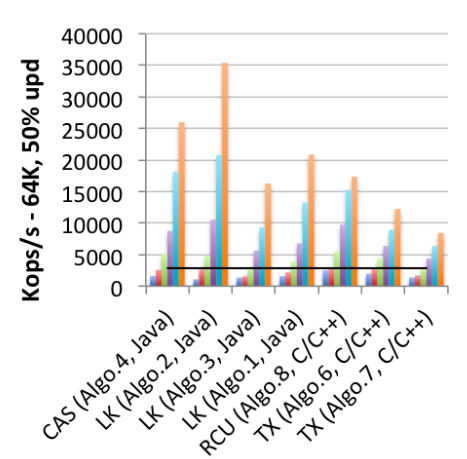
\includegraphics[scale = 0.48]{BT.png}
  \caption{Desempenho de \'{a}rvores bin\'{a}rias em ambiente concorrente. Retirado de \cite{Gramoli2015more}}
\end{figure}



\begin{figure}[htpb]
  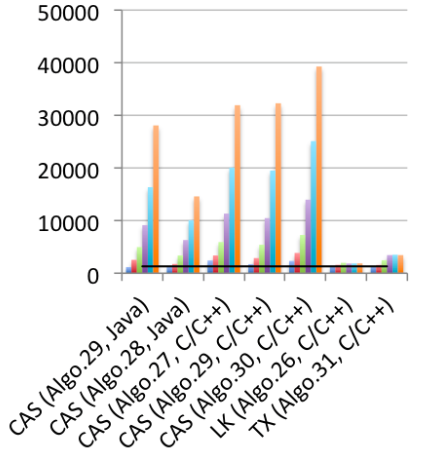
\includegraphics[scale=0.48]{SL.png}
  \caption{Desempenho de skip lists em ambiente concorrente. Retirado de \cite{Gramoli2015more}}
\end{figure}

\pagebreak

\subsection{Algumas considera\c{c}\~{o}es adicionais.} 

\begin{enumerate}

\item Em geral, no ambiente de programa\c{c}\~{a}o concorrente, os algoritmos de \textit{skip list } tem um bom desempenho em rela\c{c}\~{a}o as \'{a}rvores bin\'{a}rias;
\item De acordo com o referido artigo, a linha base (cor preta) indica o desempenho ``sem sincroniza\c{c}\~{a}o" dos algoritmos. Em primeira an\'{a}lise, observa-se que, nessa configura\c{c}\~{a}o sem sincronismo, os desempenhos em ``ops/s" dos algoritmos de \textit{skip list } s\~{a}o relativamente inferiores aos algoritmos das \'{a}rvores bin\'{a}rias. Entretanto, como visto anteriormente, na configura\c{c}\~{a}o de programa\c{c}\~{a}o concorrente, esse cen\'{a}rio muda e;
\item De acordo com \cite{Gramoli2015more}, em alguns poucos casos, alguns algoritmos de estrutura de dados  tem um desempenho relativamente baixo devido algumas sutilezas oriundas do tipo de linguagem (Java, C++, C) que foi utilizada aliada a uma determinada t\'{e}cnica de sincroniza\c{c}\~{a}o. Tais detalhamentos podem ser vistos nos itens 2.3 (\textbf{\textit{Language and memory management}}) e 4.4 (\textbf{\textit{Language effects}}) do referido artigo. 
 
\end{enumerate}

\section{Conclus\~{a}o}

As \textit{skip lists} probabil\'{i}sticas surgiram como uma alternativa as outras estruturas de dados balanceadas, tais como as \'{a}rvores bin\'{a}rias, contudo o fato mais preponderante \'{e} a relativa simplicidade da implementa\c{c}\~{a}o das \textit{skip lists} com rela\c{c}\~{a}o as outras estruturas. Em um pior caso, as skip lists podem ser tornar estruturas invi\'{a}veis. Por exemplo, caso a opera\c{c}\~{a}o de inser\c{c}\~{a}o de muitos elementos ou itens seja executada continuamente, um problema de mem\'{o}ria poder\'{a} ocorrer. Al\'{e}m disso, se todos os $n$ itens, durante esse processo de inser\c{c}\~{a}o, atingirem a altura m\'{a}xima $h$ da \textit{skip list}, ou mesmo a altura $h-1$,  a complexidade das opera\c{c}\~{o}es mudam de $O(logn)$ para $O(n + h)$. Desta forma, as skip lists determin\'{i}sticas foram criadas como uma garantia para se manter o custo das opera\c{c}\~{o}es de busca, inser\c{c}\~{a}o e remo\c{c}\~{a}o em tempo logar\'{i}tmico. 
Adicionalmente, de acordo com \cite{munro1992deterministic}, uma das raz\~{o}es da exist\^{e}ncia das \textit{skip lists} determin\'{i}sticas seria que a \textbf{redund\^{a}ncia de compara\c{c}\~{o}es} entre elementos, durante um processo de busca ou pesquisa e, muitos ponteiros, tem a vantagem de ``paralelizar uma estrutura" . Por fim, foi visto que as \textit{skip lists} podem ter um \'{o}timo desempenho em um ambiente de programa\c{c}\~{a}o concorrente em rela\c{c}\~{a}o as outras estruturas.   

%----------------------------------------------------------------------------------------
\bibliography{biblio}{}
\end{document}